
\documentclass[a4paper]{article}
\usepackage{graphicx}

\begin{document}

\section{Introduction}
This document describes how the problem of 2d-navigation was solved on a real robot.
The goal of navigation is to safely move a robot from a to b. The robot used
was moving base, the x80sv.



The task of navigation can be split up into the following tasks:

\begin{itemize}
  \item Robot control. This task is concerned with controlling the seperate wheels of the robot. Typically this is done using PID control or something alike.
  \item Odometry calculation. By keeping track of wheel motions, the robot position can be
calculated. This method is subjective to drift.
  \item Position and mapping, also known as SLAM, is the task of determining location of the robot in the world, and at the same time reconstructing the world.
  \item Global planning is the task of determining a path through a known map. This requires a search like A* or something like that.
  \item Local planning takes as input the global path and generated the appropriate motion commands for the robot control. It is some sort of setpoint generator. This layer is also responsible for obstacles. When an obstacle is observed, the path may be adjusted.
\end{itemize}

\includegraphics[width=\textwidth,height=\textheight,keepaspectratio]{img/overview.png}

The rest of this document describes all the tasks listed above as applied to the x80sv using the robot operating system (ROS).

\section{Robot setup}
The robot used in this setup is the x80sv of drrobot. This robot has three wheels, of which
two are controlled. Also standard sensors are range sensors, infrared and ultrasonic.
The robot is extended with a laser range
sensor a laptop with ROS installed. The LRS and the controllerboard of the x80sv are
connected via usb-serial cables. The controllerboard of the x80sv is provided with
the robot.

\includegraphics[width=\textwidth,height=\textheight,keepaspectratio]{img/fotorobot.png}

\section{Installation}
To use the robot, install ROS indigo on ubuntu 14.04 on the robot laptop.

Download the x80sv software from the github repository:

https://github.com/saxionled/x80sv

And follow instruction in the readme.

\section{Simulation}
Instead of trying to run everything on the real robot, a simulated version of the x80sv
was created. This was done using the gazebo simulator.

\includegraphics[width=\textwidth,height=\textheight,keepaspectratio]{img/office_sim_testgmapping.png}

\section{Control}
The velocity control is done by the controllerboard of the robot. The commands to
the controllerboard are wheel velocities in encoder ticks. A conversion from linear
and angular velocities to wheel velocities is required.

\begin{equation}
        v_{left} = (2 * v_{linear} - v_{angular} * wheelDistance) / (2 * wheelRadius)
\end{equation}
\begin{equation}
        v_{right} = (v_{angular} * wheelDistance + 2 * v_{linear}) / (2 * wheelRadius)
\end{equation}

In the next step, the wheel velocities are translated into encoder velocities.

\begin{equation}
  leftWheelCmd = -motorDir * v_{left} * encoderOneCircleCnt / (2 \pi)
\end{equation}
\begin{equation}
 rightWheelCmd = motorDir * v_{right} * encoderOneCircleCnt / (2 \pi)
\end{equation}

\section{Odometry}
The task of the odometry system is to keep track of the robot position using wheel encoder
data. To implement this for a two wheeled robot the following formulas are used:

\begin{equation}
 d_{left} = calculateMovementDelta(mtr0)
\end{equation}
\begin{equation}
 d_{right} = calculateMovementDelta(mtr1)
\end{equation}
\begin{equation}
 averageDistance = (d_{left} + d_{right}) / 2
\end{equation}
\begin{equation}
 \delta \theta = atan2((d_{right} - d_{left}), wheelDis_);
\end{equation}
\begin{equation}
 \delta x = averageDistance * cos(\theta);
\end{equation}
\begin{equation}
 \delta y = averageDistance * sin(\theta);
\end{equation}
\begin{equation}
 \theta += \delta \theta
\end{equation}
\begin{equation}
 x += \delta x
\end{equation}
\begin{equation}
 y += \delta y
\end{equation}

These are implemented in the x80 node.

\section{Slam}

For slam the standard ROS node gmapping [1] can be used.

[1] http://wiki.ros.org/gmapping

\subsection{Laser orientation}
The orientation of the laser is important for the gmapping node. The node assumes that
scan is symmetric around zero angle. This means that a laserscan message with range
0 to 2 pi will not work. A range from -pi to pi will work!

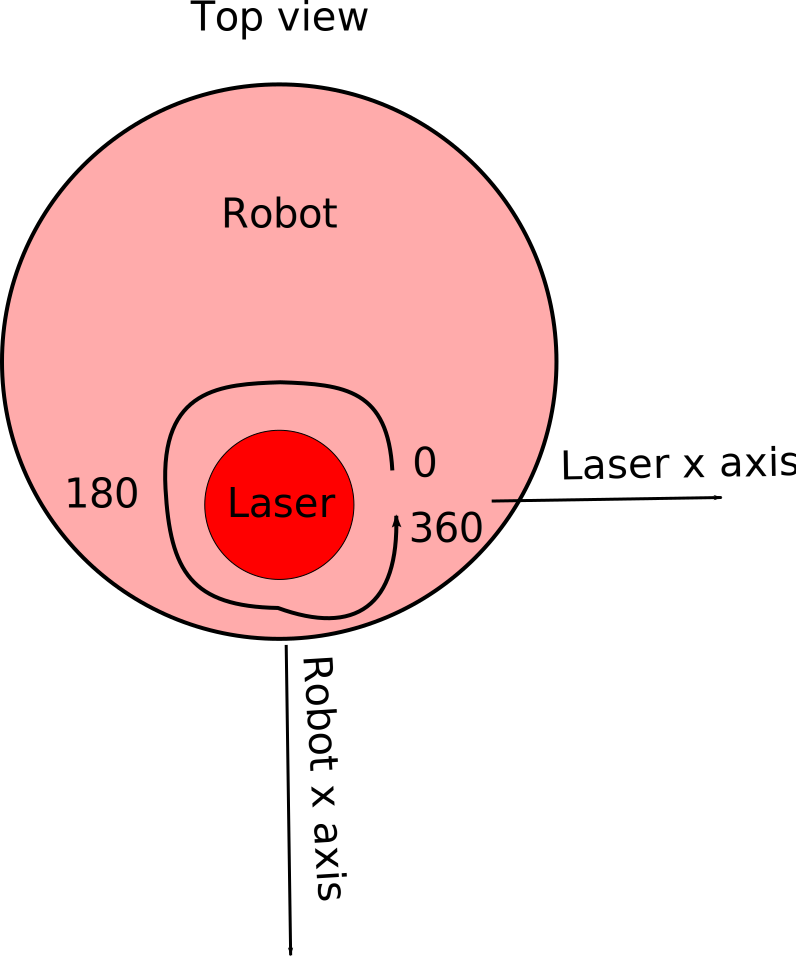
\includegraphics[width=0.5\textwidth,height=\textheight,keepaspectratio]{img/laser_orientation.png}


\section{Navigation}

\subsection{Framework}

There is an existing framework for 2d mobile base navigation:

http://wiki.ros.org/move\_base

Another framework is the skynav framework developed at saxion.


\subsection{move base}

\includegraphics[width=\textwidth,height=\textheight,keepaspectratio]{img/rviz_navigation2.png}

\section{Future work}


\end{document}

